\documentclass[10pt,a4paper,final,parskip]{scrartcl}
\usepackage[utf8]{inputenc}
\usepackage[german]{babel}
\usepackage{amsmath}
\usepackage{amsfonts}
\usepackage{amssymb}
\usepackage{graphicx}
\usepackage{lmodern}
\usepackage{paralist}
\usepackage{color}
\usepackage{tabularx} % für die erweiterten tabular Funktionen
 \usepackage{multirow}
 
\usepackage{listings,xcolor}
%\usepackage{inconsolata}
% Farben definieren
\usepackage{xcolor}
\definecolor{codeGray}{RGB}{240,240,240}
\definecolor{codeBlack}{RGB}{0,0,0}
\definecolor{codeRed}{RGB}{221,0,0}
\definecolor{codeBlue}{rgb}{0,0,187}
\definecolor{codeYellow}{RGB}{255,128,0}
\definecolor{codeGreen}{RGB}{0,119,0}

\newcommand{\blau}[1]{\textcolor{blue}{#1}}
% zum erzeugen von "todo" Zeilen
\newcommand{\todo}[1]{\colorbox{yellow}{\parbox{\textwidth}{Todo: \textbf{#1}}}}


% … und zuweisen
\lstset{%
    language=PHP,%
    %
    % Farben, diktengleiche Schrift
    backgroundcolor={\color{codeGray}},% 
    basicstyle={\small\ttfamily\color{codeGreen}},% 
    commentstyle={\color{codeYellow}},%
    keywordstyle={\color{codeBlue}},%
    stringstyle={\color{codeRed}},%
    identifierstyle={\color{codeBlue}},%
    %
    % Zeilenumbrüche aktivieren, Leerzeichen nicht hervorheben    
    breaklines=true,%
    showstringspaces=false,%
    % 
    % Listing-Caption unterhalb (bottom)
    captionpos=b,%
    % 
    % Listing einrahmen
    frame=single,%
    rulecolor={\color{codeBlack}},%
    % 
    % winzige Zeilennummern links
   % numbers=left,%
 %   numberstyle={\tiny\color{codeBlack}}%
}

\newenvironment{php}
{\begin{minipage}{\textwidth}
\begin{lstlisting}}
{\end{lstlisting}
\end{minipage}}

\newenvironment{beispiel}
{\begin{minipage}{\textwidth}
Beispiel
\begin{lstlisting}}
{\end{lstlisting}
\end{minipage}}

\begin{document}



\tableofcontents
\cleardoublepage

\section{Einrichten}
Zum Einrichten des Systems müssen einige Dinge beachtet werden, diese werden entweder hier, in nachfolgenden Kapiteln oder an ganz anderer Stelle beschrieben. Trotzdem sollen hier bereits wichtige Informationen dazu zusammengetragen werden.

\subsection{ Datenbank einspielen}
Das einspielen der Datenbank erfolgt wie im Kapitel \ref{DBEinrichten} zum Einspielen der Datenbank beschrieben.
Beachten Sie dabei, dass die dort gegebenen Datenbankdefinitionen und Beispiele für ein festes Schema/Datenbank mit dem Namen $uebungsplattform$ angelegt wurden.
Diese festen Angaben sind in de \blau{DB/Database.sql}, \blau{DB/Sample.sql} und \blau{DB/Components.sql} so vermerkt. Für den Fall, dass Sie die Datenbank mit einem anderen Namen anlegen möchten, muss dies beachtet werden.

Zum Einspielen können die in Kapitel \ref{DBEinrichten} beschriebenen Schritte/Befehle genutzt werden, oder aber
\blau{cat Database.sql Components.sql $|$ mysql} genutzt werden.
Bei Fehlern probieren Sie \blau{cat Database.sql Components.sql $|$ mysql $--$force}.

\subsection{ Datenbankzugriff einrichten}
Wie im Kapitel \ref{DBEinrichten} die Dateien für den Zugang zur Datenbank anpassen, beachten Sie dabei, wirklich alle anzupassen, jene im Ordner \blau{DB/CControl} und \blau{DB/DBQuery}.

\subsection{ Komponenten verknüpfen}
Befolgen Sie die Schritte aus dem Kapitel \ref{Verknuepfung} mittels \blau{localhost/uebungsplattform/DB/CControl/send}. Beachten Sie, dass die Komponenten (\blau{logic/...}, \blau{DB/...}) dazu in ihrem Ordner Schreibrechte benötigen, um die \blau{CConfig.json} Dateien anlegen zu können.
Die Beispielverknüpfungen der \blau{DB/Components.sql} sind für die Komponenten mit dem Basispfad \blau{localhost/uebungsplattform/} eingetragen. Sollten Ihre Komponenten im einzelnen oder in ihrer Gesamtheit einen anderen Pfad besitzen, so müssen Sie diese entsprechend Anpassen.

\subsection{Benutzeroberfläche verknüpfen}
\todo{ausfüllen}

\section{Datenbankschicht\label{Datenbankschicht}}
\begin{figure}[hptb]
  \begin{minipage}[b][7.5cm][t]{.5\linewidth}
Dieser Teil des Gesamtsystems setzt sich aus den Teilbereichen Datenbank, der dazu gehörigen Datenbankabstraktion und dem Dateisystem zusammen.\\

Dabei kann jedes Teilsystem unabhängig von den übrigen betrieben und erweitert werden. Eine Verknüpfung derer entsteht durch die entsprechende Konfiguration.\\

Um den Zugriff anderer Schichten auf das Dateisystem und die Daten\-bank\-abstraktion zu erleichtern, wurden hier sogenannte Controller als zentrale Zugangspunkte angelegt. Diese leiten eingehende Anfragen an die verantwortlichen Komponenten in ihren Teilbereichen weiter und sollten ausschließlich genutzt werden. 
  \end{minipage}
  \begin{minipage}[b]{.5\linewidth}
    \centering
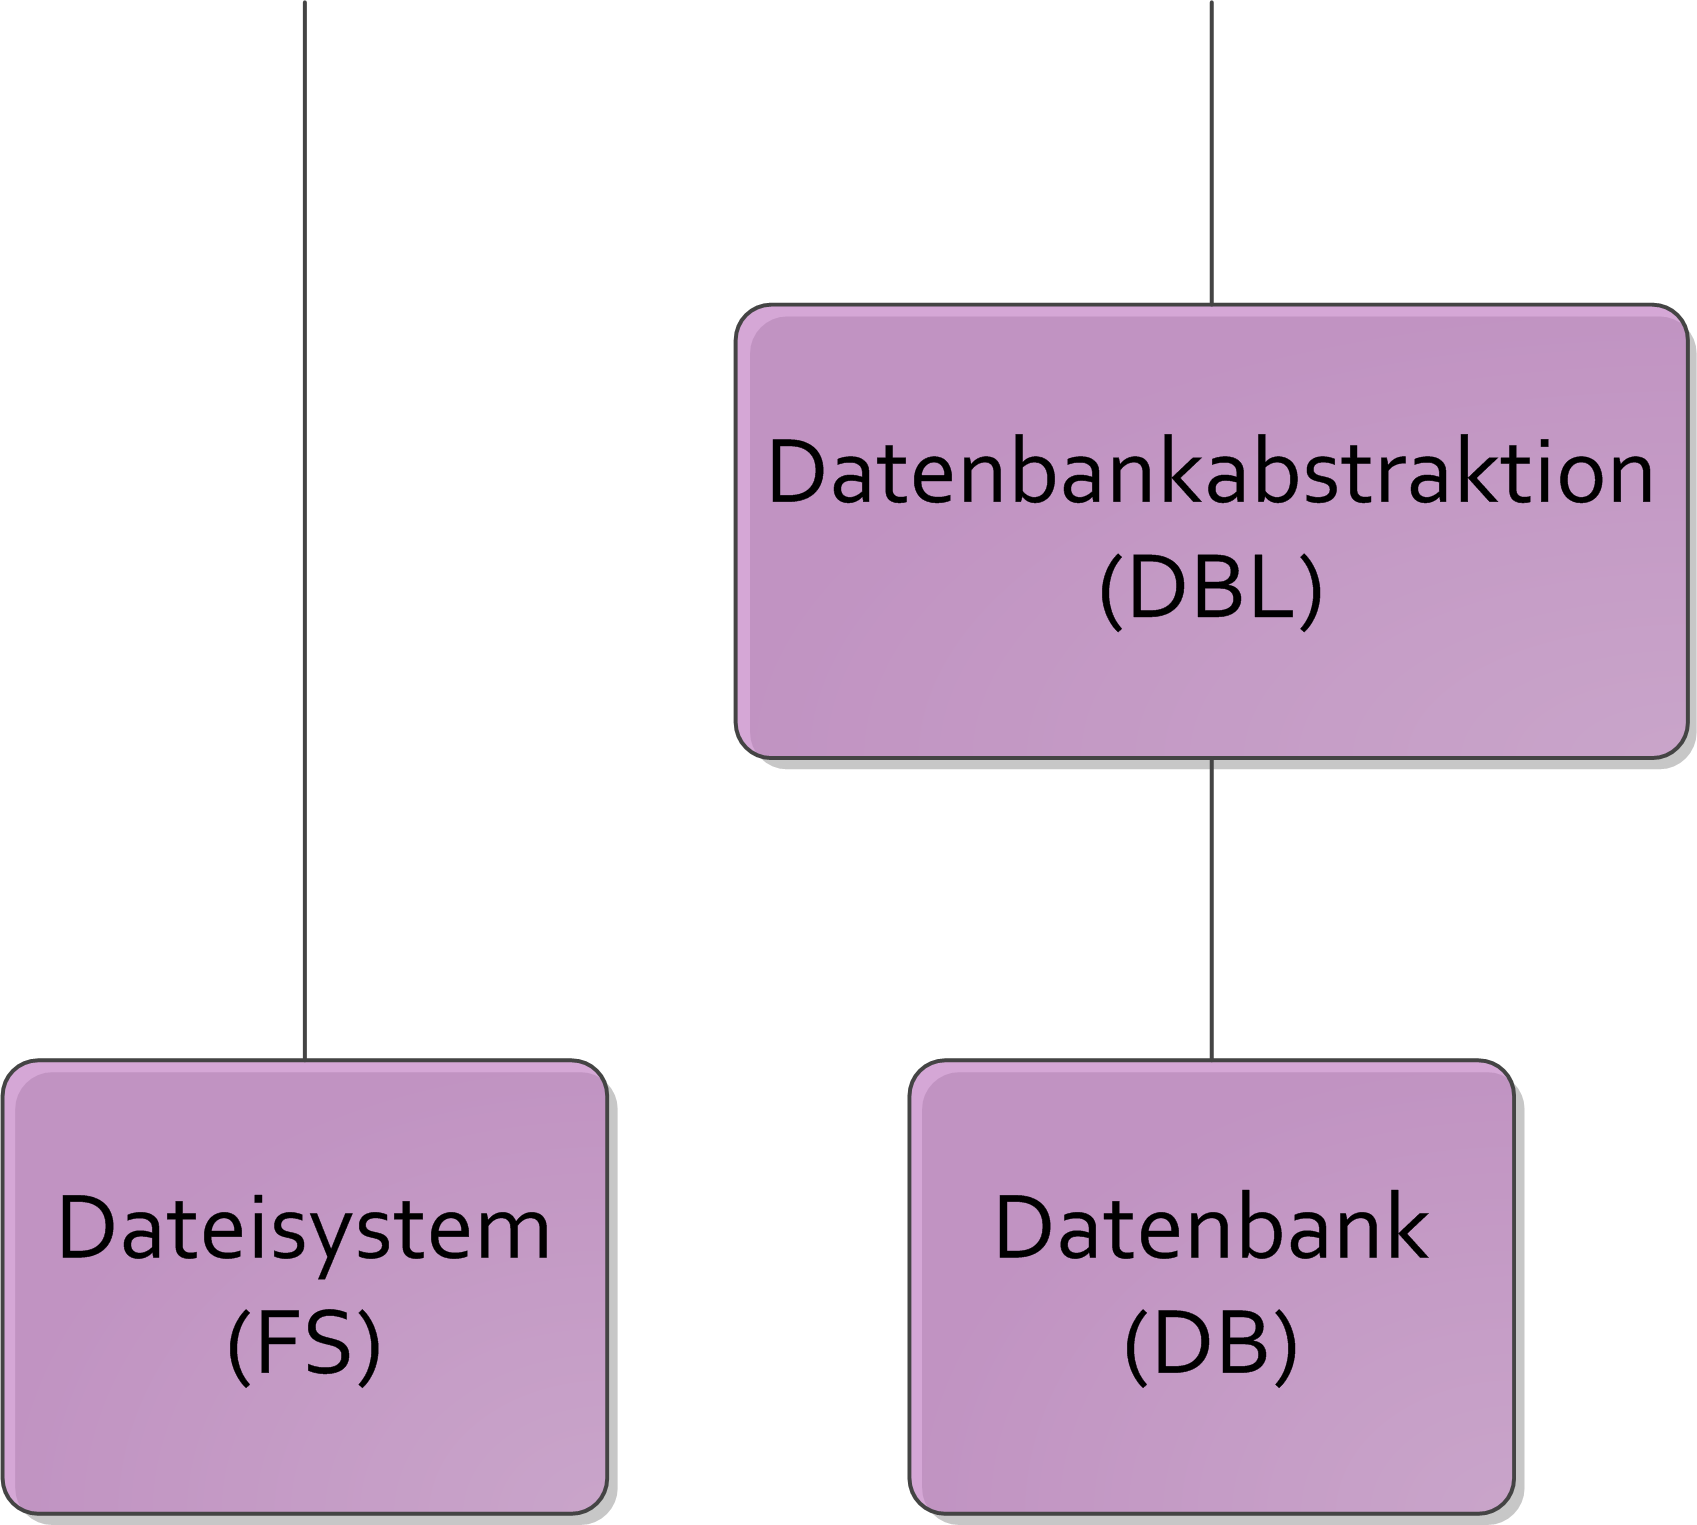
\includegraphics[scale=0.5]{Images/DB-Schichten.png}
  \end{minipage}\hfill
\end{figure}

 

\subsection{Datenbank (DB)}
\parbox{\textwidth}{Sowohl für die Speicherung der Daten, welche sich während des Betriebs der Übungsplattform ansammeln, als auch für die betriebsnotwendigen Daten wurde eine Datenbank für die Nutzung mit einem MYSQL Server unter Verwendung von MYSQL Workbench 6.0 modelliert. Dabei ergab sich ein Umfang von 19 Tabellen mit über 100 Attributen. }

\parbox{\textwidth}{Zur Beschleunigung von lesenden Anfragen wurden bei einigen Tabellen zusätzliche Attribute angelegt, wodurch die Notwendigkeit oft genutzter Join-Vorgänge minimiert wird. Der Inhalt dieser Spalten wird beim Einfügen einer neuen Datenzeile automatisch von der Datenbank mit Hilfe von implementierten Triggern befüllt, sodass diese Informationen nicht explizit angeben werden müssen.} 

\parbox{\textwidth}{Die Datenbank sollte als reiner Speicherort, ohne Wissen über den Rest des Systems, betrieben werden. Dennoch wurden aus Konsistenzgründen, zur Vereinfachung des Aufwands für andere Teilbereiche und zur Steigerung der Leistung einige Mechanismen in Form von Triggern implementiert.
Es wurden beispielsweise 35 Trigger verschiedenster Art entwickelt, um sicherzustellen, dass eine Anmeldung am System nur dann möglich ist, wenn der Nutzer nicht als gesperrt vermerkt ist.}
 
\parbox{\textwidth}{Zur Überprüfung der Langzeitstabilität des Entwurfs wurde die Datenbank während der Zeit der Entwicklung mit Beispieldaten im Umfang von rund 700.000 Datensätzen betrieben. Weiterhin wurde für eine kalkulierte Laufzeit des Systems von fünf Jahren ein lauffähiger Versuch mit über 700 Millionen Datensätzen durchgeführt.}

\parbox{\textwidth}{Zudem verwaltet die Datenbank die Verknüpfung der Komponenten der Daten\-bank\-abstraktion, des Dateisystems und der Logik-Schicht. Dafür werden ausgehende Aufrufe von Komponenten als Links bezeichnet und mit einem Namen und einer Ziel\-adresse gespeichert. Diese können dann per Aufruf über eine speziell dafür entworfene Komponente an alle im System befindlichen Komponenten verteilt werden, wodurch die zentrale Verwaltung und Konfiguration sichergestellt wird. Diese Entwurfsüberlegung ermöglicht es, das Weiterleitungsverhalten einzelner Komponenten zentral zu verändern und im Bedarfsfall zusätzliche Komponenten an entsprechenden Stellen einzuhängen, um so das System zu erweitern.}


\subsection{Datenbankabstraktion (DBL)}
\parbox{\textwidth}{Um den Zugang zur Datenbank zu vereinfachen und den direkten Zugriff über SQL Befehle zu vermeiden, wurde eine Vereinfachung entwickelt, welche feste Befehle nach außen über eine mittels Slim umgesetzte REST-API zur Verfügung stellt. Dazu wurden zusätzlich Datenstrukturen für die inhaltliche Darstellung und Kommunikation von Objekten entworfen, welche die DBL in Form eines JSON-konformen Objekts erwartet und in ihren Antworten ebenso auch kodiert.}

\parbox{\textwidth}{Die Anfragen werden nach dem Eintreffen in SQL Befehle übersetzt und mit einer der DBL zur Verfügung gestellten Datenbankschnittstelle umgesetzt.}

\parbox{\textwidth}{Dieses Vorgehen, welches direkte Datenbankzugriffe unterbindet, steigert die Austauschbarkeit sowie die einfache Erweiterbarkeit der Befehlsvielfalt. Außerdem wird an dieser Stelle sichergestellt, dass die Abfragen festgelegte Bedingungen erfüllen, wie beispielsweise die Einhaltung eines bestimmten Datentyps für Parameter des REST-Aufrufs. Darüber hinaus werden eingehende Daten von unerlaubten Inhalten bereinigt, um einen nicht ordnungsgemäßen Zugriff auf innere Systeme sowie Datenbestände zu verhindern.}

\parbox{\textwidth}{Um ein umfangreiches Angebot unterschiedlichster Anfragen an die Datenbank bereitstellen zu können, wurde ein Verbund aus 20 unabhängigen Komponenten mit über 140 Befehlen entwickelt, wobei eine  Komponente im Allgemeinen für die Bereitstellung von Funktionen zur Handhabung der entsprechenden Tabelle der Datenbank zuständig ist.}

\parbox{\textwidth}{Zur Sicherstellung der korrekten Funktionalität der Komponenten wurden einfache, automatisierte Tests unter Verwendung des PHPUnit Frameworks entworfen, durch welche die Komponenten in ihrer Gesamtheit auf die Erfüllung von über 400 Bedingungen geprüft werden können. Es muss jedoch angemerkt werden, dass diese Tests keine ausführliche Prüfung der Funktionalität der Komponenten darstellen.}

\subsection{Dateisystem (FS)}
\parbox{\textwidth}{Zur Speicherung von Dateiinhalten -- wie beispielsweise die von Studenten eingereichten Lösungen zu Übungsaufgaben -- wurden fünf weitere Komponenten entwickelt. Diese sind für die Verwaltung gespeicherter Inhalte, die Wahl des Speicherortes und der Erstellung von Archiven im ZIP-Format aus gespeicherten Inhalten zuständig. }

\parbox{\textwidth}{Es war dabei ein wesentliches Anliegen, dass die redundante Speicherung von Dateiinhalten vom Dateisystem selbstständig verhindert wird. Dies geschieht durch die Benennung der gespeicherten Dateien anhand des SHA1-Hashs, welcher von der entsprechenden Datei gebildet wird.}

\parbox{\textwidth}{Das Dateisystem behandelt die Dateiinhalte, ohne dabei die Herkunft oder die Bedeutung der Dateien kennen zu müssen. Zusätzlich ist es bereits in der Lage, die zu speichernden Inhalte per Konfiguration auf mehrere Speicherorte gleichmäßig zu verteilen, was durch die Entscheidung, einen Hash als Speichernamen zu verwenden, ermöglicht wurde.}


\subsection{Sicherheitskonzept der Datenbankschicht}
Die Datenbankschicht kann lediglich sicherstellen, dass die Informationen die eingehen, nicht dieser Schicht schaden können. Dabei kann nicht sichergestellt werden, das die Aufrufe, die an sie gestellt werden für den Nutzer erlaubt sind. Sodass jemand eine korrekte Abfrage zum Abrufen aller Nutzerdaten formulieren könnte, ohne das sich die Datenbankschicht daran stört.

\subsubsection{Datenbank}
Die SQL Anfragen, welche an der Datenbank eintreffen, müssen bereits korrekt sein und werden an dieser Stelle nicht weiter geprüft. Daher sollten Anfragen lediglich über die $DBQuery$ mithilfe der $Query$ Datenstruktur, an die Datenbank gestellt werden.

\subsubsection{Datenbankabstraktion}
Der Schutz der Datenbank vor unerlaubten Zugriffen, sowie der Ausführung nicht erlaubter Befehle wird innerhalb dieses Bereichs sichergestellt.

Dabei werden eingehende Daten für POST und PUT Zugriffe durch die \blau{getInsertData()} Funktionen der Datenstrukturen maskiert, um unerlaubte Zeichen innerhalb der Daten zu unterbinden. Dazu wird die \blau{DBJson::mysql\_real\_escape\_string()} Funktion genutzt.

\begin{minipage}{\textwidth}
\begin{lstlisting}
...
if ($this->id != null) 
    $this->addInsertData(
        $values, 
        'C_id',
        DBJson::mysql_real_escape_string($this->id));
...
\end{lstlisting}
\end{minipage}

Informationen die über die REST Aufrufe zu den Komponenenten gelangen, beispielsweise \blau{/DB/DBControl/course/1}, werden ebenfalls, sofern sie beliebige Daten enthalten können, maskiert. 

\begin{minipage}{\textwidth}
\begin{lstlisting}
...
$userid = DBJson::mysql_real_escape_string($userid);
...
\end{lstlisting}
\end{minipage}

Da die meisten dieser Aufrufe jedoch nur Ziffern als Eingabe erwarten, wird auch eine Prüfung mit \blau{ctype\_digit()} in diesen Fällen vorgenommen und im Falle unerlaubter Eingaben der Fehlercode 412 von der Komponente zurückgegeben.

\begin{minipage}{\textwidth}
\begin{lstlisting}
...
DBJson::checkInput($this->_app, 
                   ctype_digit($courseid));
...
\end{lstlisting}
\end{minipage}

Desweiteren werden Anfragen nur über die $DBQuery$ Komponente mit Hilfe der $Query$ Datenstruktur an die Datenbank gestellt, dabei steuert das $checkSession$ Flag der $Query$ Datenstruktur ob die $DBQuery$ Komponente vor der Ausführung der SQL Anfrage prüfen soll, ob eine gültige Session in der Datenbank vermerkt wurde. 

Bei der Prüfung auf eine gültige Session werden die Headerfelder \blau{HTTP\_SESSION}, \blau{HTTP\_USER} und \blau{HTTP\_DATE} genutzt und auf ihre Gültigkeit mithilfe der $Session$ Tabelle der Datenbank geprüft. Wird dabei die Anfrage abgelehnt, so wird die Anfrage abgebrochen und der Fehlercode 401 zurückgegeben. Diese Prüfung findet innerhalb der \blau{request()} Funktion der \blau{Assistants/DBRequest.php} statt.

Zudem erlaubt die $DBQuery$ Komponente nur eine einzige SQL Anfrage pro $Query$ Struktur im $request$ Feld.

\subsubsection{Dateisystem}
Das Dateisystem schützt den Zugriff auf seine Dateien lediglich dadurch, das für das Abrufen die genaue Adresse, welche auf dem SHA1-Hash der Datei basiert bekannt sein muss.
Bsp.: \blau{file/757097c90146e7ad82aceb68015943ac090ca6b4}.

Diese Lösung macht die Arbeit des Dateisystems sehr einfach, da es keinerlei Informationen darüber besitzen muss, wem die Datei gehört und welchem Zweck sie dient. Gleichzeitig ist es aber auch nicht möglich, anhand der Datei irgendwelche Aussagen über den Originalnamen, den Dateityp (sofern nicht aus dem Inhalt bestimmt), den Zweck, sowie den Besitzer zu treffen.

\subsection{Datenbank Entwurfsgrundlagen}
Um die Belastung einzelner Tabellen und das ausmaß der Einträge einschätzen zu können, wurden Schätzungen aufgestellt, welche die Anzahl der Einträge in der Datenbank für 5 Jahre vorhersagbar machen sollen. Diese Zahlen bilden auch die Grundlage für den Entwurf der Beispieldaten, die während der Entwicklung genutzt wurden.

\subsubsection{Mit wievielen Einträgen muss gerechnet werden?}
 \begin{tabular}{p{.40\textwidth}p{.15\textwidth}p{.35\textwidth}}
Bereich  & Menge  & Bedarf \\
\hline
\multirow{2}{.40\textwidth}{Nutzer pro \\ Veranstaltung} & \multirow{2}{.15\textwidth}{80} & \multirow{2}{.35\textwidth}{80 Veranstaltungsteilnahmen} \\ && \\\hline

\multirow{3}{.40\textwidth}{Übungsserien pro\\ Veranstaltung } & \multirow{3}{.15\textwidth}{15} &15 Übungsserieneinträge\\
& & 15 Aufgabenblätter \\
& & 15 Musterlösungsdateien\\\hline

\multirow{2}{.40\textwidth}{Aufgaben pro \\ Übungsserie}& \multirow{2}{.15\textwidth}{5} & \multirow{2}{.35\textwidth}{5 Aufgaben} \\ && \\\hline

\multirow{2}{.40\textwidth}{Anhänge pro \\ Übungsserie} & \multirow{2}{.15\textwidth}{1,5} & 1,5 Anhänge \\
&& 1,5 Anhangsdateien\\\hline

\multirow{2}{.40\textwidth}{Zulassungsbedingungen pro \\ Veranstaltung} & \multirow{2}{.15\textwidth}{2} & \multirow{2}{.35\textwidth}{2 Zulassungsbedingungen} \\ && \\\hline

\multirow{2}{.40\textwidth}{Gruppen pro \\ Übungsserie} & \multirow{2}{.15\textwidth}{80} & \multirow{2}{.35\textwidth}{80 Gruppeneinträge} \\ && \\\hline

\multirow{3}{.40\textwidth}{Einsendungen pro \\ Nutzer pro \\ Aufgabe} & \multirow{3}{.15\textwidth}{1,2} & 1,2 Einsendungen \\
&& 1,2 Einsendungsdateien \\ && \\\hline

\multirow{3}{.40\textwidth}{Korrekturen pro \\ Aufgabe pro \\ Nutzer}  & \multirow{3}{.15\textwidth}{0,8}  & 0,8 Korrektureinträge  \\
 &  & 0,8 Korrekturdateien\\&&\\\hline

 
\multirow{2}{.40\textwidth}{Veranstaltungen pro \\ Semester}  &  \multirow{2}{.15\textwidth}{2500}  &  \multirow{2}{.35\textwidth}{2500 Veranstaltungseinträge}\\ && \\\hline

Nutzungsdauer & 5 Jahre & 10 Semester \\
\end{tabular}

\subsubsection{Womit müssen wir rechnen?}
Daraus ergibt sich die folgende Anzahl an Datenbankeinträgen für die entsprechenden Tabellen:

 \begin{tabular}{l>{$}r<{$}}
Tabelle & $Zeilenanzahl$ \\
\hline
Nutzer(User) & 100.000 (festgelegt) \\
Veranstaltungen(Course) & 25.000 \\
Übungsserien(ExerciseSheet) & 375.000 \\
Aufgaben(Exercise) & 1.875.000 \\
Anhänge(Attachment) & 562.500 \\
Dateien(File) & 301.312.000 \\
Zulassungsbedingungen(ApprovalCondition) & 50.000 \\
Gruppen(Group) & 30.000.000 \\
Einsendungen(Submission) & 180.000.000 \\
Korrekturen(Marking) & 120.000.000 \\
Veranstaltungsteilnahmen(CourseStatus) & 2.000.000 \\
Aufgabensorten(ExerciseType) & 20 (festgelegt) \\
ausgewählte Einsendungen(SelectedSubmission) & 120.000.000 \\
 \end{tabular}
 
 \subsection{Datenbank einrichten\label{DBEinrichten}}
 \subsubsection{Dateien}
  \begin{tabular}{l>{$}r<{$}}
  \multirow{1}{.20\textwidth}{Database.mwb} & 
 \multirow{1}{.70\textwidth}{MySQL Workbench Modell, MySQL Workbench Diagramm} \\\hline

\multirow{7}{.20\textwidth}{Database.sql} & \multirow{7}{.70\textwidth}{Enthält die aus \blau{Database.mwb} generierte SQL Datenbankdefinition. Diese Datei erstellt eine Datenbank mit dem Namen $uebungsplattform$, sofern eine solche Datenbank bereits existiert, wird die bereits existierende zuvor entfernt. Das einspielen erfolgt über die Konsole nach dem einloggen bei $mysql$ mittels \blau{source Database.sql} oder mit Hilfe von PHPMyAdmin, über $import$.}\\&\\&\\& \\&\\&\\&\\\hline

\multirow{7}{.20\textwidth}{Insert.sql} & \multirow{7}{.70\textwidth}{Enthält Beispieldaten für die Datenbank, diese werden auch für die Testszenarien genutzt. Das einspielen erfolgt entweder überden PHPMyAdmin mit $import$ oder über die Konsole mit \blau{mysql uebungsplattform $<$ Insert.sql} (http://dev.mysql.com/doc/refman/5.0/en/mysql-batch-commands.html)}\\&\\& \\&\\&\\& \\&\\
 \end{tabular}
 
   Zusätzlich gibt es die Datei \blau{DB/Components.sql}, diese enthält Beispielverknüpfungen für die Datenbank $uebungsplattform$ und muss ebenfalls eingespielt oder aber abgeändert werden.


\subsubsection{Software}
  \begin{tabular}{l>{$}r<{$}}
\multirow{2}{.20\textwidth}{MySQL Server} & \multirow{2}{.70\textwidth}{Zum Betreiben der Datenbank (http://dev.mysql.com/downloads/mysql/)}\\& \\ \hline
\multirow{2}{.20\textwidth}{MySQL Workbench} & \multirow{2}{.70\textwidth}{Zum Bearbeiten der Database.mwb (http://www.mysql.de/products/workbench/)}\\&\\
 \end{tabular}
 
\subsubsection{Einstellungen}
Zum betreiben der DB Komponenten müssen die Datenbankzugangsdaten bei den Komponenten $CControl$ und $DBQuery$ in die entsprechenden \blau{config.ini} Dateien Eingetragen werden.

\blau{DB/CControl/config.ini} und 
\blau{DB/DBQuery/config.ini}

Beispielinhalt der beiden config.ini Dateien:

\begin{minipage}{\textwidth}
\begin{lstlisting}
[DB]
db_path = localhost // Pfad zum Ansprechen der Datenbank
db_user = root // der Nutzername des Zugangs
db_passwd = test // das Passwort des Zugangs
db_name = uebungsplattform //  der Datenbankname (Database.sql 
                           // nutzt den Datenbanknamen
                           // "uebungsplattform")
\end{lstlisting}
\end{minipage}

Damit wir mit deutschen Umlauten in unserer Datenbank arbeiten können, muss die \blau{my.cnf} bzw. \blau{my.ini} des MySQL-Server angepasst werden.

\begin{minipage}{\textwidth}
my.cnf oder my.ini
\begin{lstlisting}
[client]
#
# nicht auf utf-8 einstellen!!
#

[mysql]
#
# Standardeinstellung war leer, scheint zu funktionieren.
#

[mysqld]

character_set_server=utf8
skip-character-set-client-handshake
...
\end{lstlisting}
\end{minipage}

\section{Datenstrukturen}
Die meisten Datenstrukturen werden unter
\textcolor{blue}{Assistants/Structures.php} beschrieben, dabei gibt es einige grundlegende Operationen die eine solche Datenstruktur zur Verfügung stellt.

Diese sollen hier am Beispiel der $Course$ Datenstruktur in der Datei \textcolor{blue}{Assistants/Structures/Course.php} erklärt werden.

\subsection{Attribute}
\begin{minipage}{\textwidth}
\begin{lstlisting}
private $id = null;

    public function getId()
    {
        return $this->id;
    }
    
    public function setId($value)
    {
        $this->id = $value;
    }
\end{lstlisting}
\end{minipage}

Jedes Attribut wird als eigene Variable mit default Wert definiert, dieser wird bei der Übertragung ignoriert, sodass default Werte nicht nutzlos übertragen werden. Zudem sollten $get$ und $set$ Funktionen für die Attribute entworfen und genutzt werden.

\begin{minipage}{\textwidth}
Beispiel:
\begin{lstlisting}
$obj = new Course();
$obj->setId(2);
echo $obj->getId();
// Ausgabe: 2
\end{lstlisting}
\end{minipage}

\subsection{Objekte für PUT und POST erstellen}
\begin{minipage}{\textwidth}
\begin{lstlisting}
    public static function createCourse($courseId,$name,$semester,$defaultGroupSize)
    {
    	...
    }
\end{lstlisting}
\end{minipage}

Um das erstellen neuer Objekte für eine Course Datenstruktur zu erleichtern, wurden $create$ Funktionen entworfen, diese nehmen die möglichen in die Datenbank eintragbaren Attribute entgegen und bringen sie in eine Form, mit der die Datenbank bei PUT und POST arbeiten kann.

Es wird ein Course Objekt zurückgegeben. Dieses kann mit \textcolor{blue}{Course::encodeCourse()} oder \textcolor{blue}{json\_encode()} zum Versand in einem HTTP Request mittels JSON vorbereitet werden.

Will man den default-Wert der Datenbank bei einem POST Befehl für seinen Eintrag nutzen oder ein Attribut bei einem PUT im Originaleintrag nicht ändern, so wird beim Aufruf der \blau{createCourse()} Funktion an der entsprechenden Stelle \blau{null} notiert. 

\begin{minipage}{\textwidth}
Beispiel:
\begin{lstlisting}
$obj = Course::createCourse(1,'AAA','09/10',null);
echo $obj->getId();
// Ausgabe: 1

$result = Request::post('DBCourse/course',
                        array(),
                        Course::encodeCourse($obj));
\end{lstlisting}
\end{minipage}

\subsection{Datenbankattributnamen in Datenstrukturnamen konvertieren}
\begin{minipage}{\textwidth}
\begin{lstlisting}
  public static function getDbConvert()
    {
    	...
    }
\end{lstlisting}
\end{minipage}

Um zwischen den Bezeichnungen der Datenbank und denen der allgemein genutzten Datenstrukturen umwandeln zu können, gibt diese Funktion ein assoziatives Array zurück. 

Dabei ist es möglich das einige Konvertierungen nicht real in der Datenbank existieren, dieser Fall tritt ein, wenn die Datenstruktur beispielsweise vorsieht, dass $Course$ Objekte eine Liste von ExerciseSheets enthalten soll, dazu gibt es dann in der $Course$ Datenstruktur den Eintrag:
 
\begin{minipage}{\textwidth}
\begin{lstlisting}
'C_exerciseSheets' => 'exerciseSheets'
\end{lstlisting}
\end{minipage}

Dieser wird von den Komponenten genutzt und ist vorallem vorgesehen um das ganze exakt zu beschreiben.

\begin{minipage}{\textwidth}
Beispiel:
\begin{lstlisting}
echo Course::getDbConvert()['C_id'];
// Ausgabe: id
\end{lstlisting}
\end{minipage}

\subsection{Primärschlüssel der Datenbanktabellen}
\begin{minipage}{\textwidth}
\begin{lstlisting}
    public static function getDbPrimaryKey()
    {
    	...
    }
\end{lstlisting}
\end{minipage}

Die \blau{getDbPrimaryKey()} Funktionen liefern die Primärschlüssel der Tabellen entweder als einzelnen String, wenn der Primärschlüssel nicht aus mehreren Attributen besteht und als Array, wenn er sich aus mehreren Attributen zusammensetzt.

\begin{minipage}{\textwidth}
Beispiel:
\begin{lstlisting}
echo Course::getDbPrimaryKey();
// Ausgabe: C_id
\end{lstlisting}
\end{minipage}

\subsection{PUT und POST Daten aus Objekten erstellen}
\begin{minipage}{\textwidth}
\begin{lstlisting}
    public function getInsertData()
    {
    	...
    }
\end{lstlisting}
\end{minipage}

Die \blau{getInsertData()} Funktionen wandeln ein Objekt in für SQL Anfragen nutzbare Zuweisungen um.

Dabei liefert die Funktion einen String zurück.

\begin{minipage}{\textwidth}
Beispiel:
\begin{lstlisting}
echo Course::getInsertData();
// Ausgabe: C_id = '1', C_name= 'AAA', C_semester = '09/10'
\end{lstlisting}
\end{minipage}

\subsection{Konstruktor}
\begin{minipage}{\textwidth}
\begin{lstlisting}
    public function __construct($data=array())
    {
    	...
    }
\end{lstlisting}
\end{minipage}

Der Konstruktor soll entweder ein leeres Objekt mit den default Werten oder direkt aus einem assoziativen Array heraus erzeugen.

\begin{minipage}{\textwidth}
Beispiel:
\begin{lstlisting}
$obj = new Course();
echo $obj->getId();
// Ausgabe: null

$obj = new Course(array(
                 'id' => '1',
                 'name' => 'AAA'));
 echo $obj->getId();
// Ausgabe: 1
\end{lstlisting}
\end{minipage}

\subsection{ein Objekt in JSON umwandeln}
\begin{minipage}{\textwidth}
\begin{lstlisting}
    public static function encodeCourse($data)
    {
    	...
    }
\end{lstlisting}
\end{minipage}

Um ein Objekt der Datenstrukturen zu serialisieren wird die \blau{encodeCourse()} Funktion genutzt. Sie wandelt ein Objekt in einen validen JSON-String um.

\begin{minipage}{\textwidth}
Beispiel:
\begin{lstlisting}
$obj = Course::createCourse(1,'AAA','09/10',null);
echo Course::encodeCourse($obj);

// Ausgabe: 
//	{
//           "id": "1",
//           "name": "AAA",
//           "semester": "09/10"
//	}
\end{lstlisting}
\end{minipage}

\subsection{ein Objekt aus JSON erstellen}
\begin{minipage}{\textwidth}
\begin{lstlisting}
    public static function decodeCourse($data, $decode=true)
    {
    	...
    }
\end{lstlisting}
\end{minipage}

Diese Funktion wandelt JSON-Daten die ein oder mehrere Objekte darstellen können und dabei auch Unterobjekte enthalten können, in ein Objekt der Datenstruktur um. So könnte beispielsweise ein $Submission$ Objekt zusätzlich ein angehängtes $File$ Objekt besitzen, dieses wird an dieser Stelle ebenfalls dekodiert, mit der \blau{File::decodeFile()} Funktion und an die $Submission$ angehängt.

\begin{minipage}{\textwidth}
Beispiel:
\begin{lstlisting}
$data = '{"id": "1","name": "AAA","semester": "09/10"}';
$obj = Course::decodeCourse($data);
echo $obj->getId();
// Ausgabe: 1

$data = '[{"id": "1","name": "AAA","semester": "09/10"},
          {"id": "2"}]';
$obj = Course::decodeCourse($data);
echo $obj[1]->getId();
// Ausgabe: 2
\end{lstlisting}
\end{minipage}

\subsection{JSON Serialisierung}
\begin{minipage}{\textwidth}
\begin{lstlisting}
    public function jsonSerialize() 
    {
    	...
    }
\end{lstlisting}
\end{minipage}

Um Objekte dieser Datenstruktur mit \blau{Course::encodeCourse()} zu serialisieren, wird eine \blau{jsonSerialize()} Funktion benötigt, die festlegt, welche Attribute umgewandelt werden und welche nicht. 

Diese Funktion wird nicht direkt Aufgerufen.

\subsection{Objekte aus einer Datenbankantwort extrahieren}
\begin{minipage}{\textwidth}
\begin{lstlisting}
    public static function ExtractCourse($data, $singleResult = false)
    {
    	...
    }
\end{lstlisting}
\end{minipage}

Datenbankantworten, die als assoziatives Array vorliegen, werden mit dieser Funktion in assoziative Arrays umgewandelt, die der Datenstruktur entsprechen, diese können als Objekte der Datenstruktur genutzt werden, um sie dann beispielsweise zu serialisieren.

\begin{minipage}{\textwidth}
Beispiel:
\begin{lstlisting}
$res = Course::ExtractCourse(
                             array(
                                   array(
                                         'id' => '1',
                                         'name' => 'AAA'
                                   )
                             ),
                             true);
echo Course::encodeCourse($obj);

// Ausgabe: 
//	{
//           "id": "1",
//           "name": "AAA",
//           "semester": "09/10"
//	}
\end{lstlisting}
\end{minipage}

\begin{minipage}{\textwidth}
Beispiel 2:
\begin{lstlisting}
$res = Course::ExtractCourse(
                             array(
                                   array(
                                         'id' => '1',
                                         'name' => 'AAA'
                                   )
                             ),
                             false);
echo Course::encodeCourse($obj);

// Ausgabe: 
//  [
//	    {
//               "id": "1",
//               "name": "AAA",
//               "semester": "09/10"
//	    }
//  ]
\end{lstlisting}
\end{minipage}
 
 \section{Komponenten}
 
 \subsection{Verknüpfung\label{Verknuepfung}}%
Die Verknüpfung der Komponenten erfolgt zentral aus der Datenbank heraus, dort gibt es die Tabelle $Component$ und $ComponentLinkage$, diese definieren die Orte der Komponenten und die Verknüpfung derer. Dabei können lediglich Aufrufe definiert werden. Ein $Link$ zwischen zwei Komponenten A, als Besitzer des Links und B als Ziel des Links, stellt damit einen Aufruf von A nach B dar.

Beispiele für eine solche Verknüpfung befinden sich in der Datei \blau{DB/Components.sql}.
Diese sind fest für die Datenbank $uebungsplattform$ angelegt, sofern Sie eine andere Datenbank nutzen möchten, ändern Sie diese Bezeichnung.

\begin{minipage}{\textwidth}
Beispiel eines Komponenteneintrages der Tabelle $Component$
\begin{lstlisting}
...
INSERT INTO `uebungsplattform`.`Component` 
(`CO_id`, `CO_name`, `CO_address`, `CO_option`) VALUES 
(1, 'FSControl', 'localhost/uebungsplattform/FS/FSControl', '');
...
\end{lstlisting}
\end{minipage}

\begin{minipage}{\textwidth}
Beispiel eines Verlinkungseintrages der Tabelle $ComponentLinkage$
\begin{lstlisting}
...
INSERT INTO `uebungsplattform`.`ComponentLinkage` 
(`CL_id`, `CO_id_owner`, `CL_name`, `CL_relevanz`, `CO_id_target`) 
VALUES (1, 3, 'getFile', '', 1);
...
\end{lstlisting}
\end{minipage}


Dazu wurde eine Komponente $CControl$ in \blau{DB/CControl} entwickelt. Diese stellt Funktionen bereit, um die Definitionen in die Datenbank einzutragen und zu entnehmen.

Mit Hilfe des Aufrufs \blau{DB/CControl/send} entnimmt die Komponente CControl die Definitionen aus der DB und versendet sie an alle betroffenen Komponenten. 

Die Ausgabe eines solchen Aufrufs könnte folgendermaßen aussehen: \\
\blau{201--FSControl--localhost/uebungsplattform/FS/FSControl}\\
\blau{201--FSFile--localhost/uebungsplattform/FS/FSFile}\\
\blau{201--FSZip--localhost/uebungsplattform/FS/FSZip}\\
\blau{201--DBControl--localhost/uebungsplattform/DB/DBControl}\\
\blau{201--FSBinder--localhost/uebungsplattform/FS/FSBinder}\\
...\\

Dabei stehen links die HTTP Statuscodes der Antworten der Komponenten, mittig der Name der Komponenten aus der Datenbank und rechts die Adresse, welcher die Definition geschickt wurde.

Dabei nehmen die Komponenten diese Informationen entgegen und legen in ihrem Ordner \blau{CConfig.json} Dateien an.
Diese Enthalten die Informationen über die Komponenten selbst und die Informationen über die definierten Links.

\begin{minipage}{\textwidth}
\begin{lstlisting}
{
    "id": "6",
    "name": "DBCourse",
    "address": "localhost/uebungsplattform/DB/DBCourse",
    "option": "",
    "prefix": "course",
    "links": [
        {
            "id": "6",
            "name": "out",
            "address": "localhost/uebungsplattform/DB/DBQuery",
            "target": "13",
            "prefix": "query",
            "owner": "6",
            "relevanz": ""
        }
    ]
}
\end{lstlisting}
\end{minipage}

Diese Informationen können mit der, in der Datei \blau{Assistants/CConfig.php} definierten Klasse $CConfig$ in der Komponenten genutzt werden.
Dazu sollte am besten noch vor dem Aufrufen der eigentlichen Komponente ein Objekt dieser Klasse erstellt und mit entsprechenden Informationen versorgt werden. So kann jede Komponente für sich einen Präfix vergeben, auf den sie reagiert. Sollte sie keinen bestimmten Präfix verlangen, so wird ein leerer String '' angegeben, bei der Nutzung mehrerer werden diese durch Komma getrennt.

Das CConfig Objekt enthält selber einen Slim Aufruf, der prüft ob die Komponente mit $/component$ aufgerufen wurde, in diesem Falle würde die Komponente mit eingehenden Definitionsdaten oder dem Abrufen derer rechnen.

Um die Verknüpfung in einer Komponente umzusetzen, könnte man folgendermaßen vorgehen.

\begin{minipage}{\textwidth}
\begin{lstlisting}
include_once( '../../Assistants/CConfig.php' );
...
// erstellt das CConfig Objekt und teilt allen anderen mit,
// dass diese Komponenten auf den Praefix course reagiert
$com = new CConfig(course);

// Wenn es keinen '/component' Aufruf gab, kann die eigentliche
// Komponente DBCourse geladen werden.
if (!$com->used())
    new DBCourse());
  
\end{lstlisting}
\end{minipage}

Möchte man nun die Links in seiner Komponente nutzen, so müssen sie zunächst aus der \blau{CConfig.json} geladen werden mit \blau{\$com-$>$loadConfig()}.

\begin{minipage}{\textwidth}
\begin{lstlisting}
...
// laedt die CConfig.json
$conf = $com->loadConfig() ;

// laedt ein Array von Link Objekten in $links
$links = $conf->getLinks(); 
\end{lstlisting}
\end{minipage}

Weitere Informationen über den Aufbau der Component und der Link Datenstruktur können den \blau{Assistants/Structures/Component.php} und \blau{Assistants/Structures/Link.php} Dateien entnommen werden.

Wichtig ist noch zu wissen, dass die Komponenten, wenn sie die Definitionen empfangen haben, nicht wissen, welchen Präfixe die Komponenten besitzen, mit denen sie verknüpft sind. Dazu werden sie bei jedem Aufruf prüfen, ob sie alle Präfixe kennen und in dem Fall, in dem sie einen Präfix nicht kennen, diesen von der entsprechenden Komponente abfragen.

Sollte es also zu langen Wartezeiten beim Aufrufen von Komponenten kommen, sollte geprüft werden, ob die Komponente alle ihre Ziele erreichen kann oder sie eventuell vergebens versucht diese zu kontaktieren.

 \subsection{Testen}
 Für den größten Teil der Komponenten wurden einfache Tests entwickelt, um PHP Syntaxfehler zu verhindern. 
 
  \subsubsection{Dateien}
 \begin{tabular}{l>{$}r<{$}}

\multirow{7}{.20\textwidth}{Database.sql} & \multirow{7}{.70\textwidth}{Enthält die aus \blau{Database.mwb} generierte SQL Datenbankdefinition. Diese Datei erstellt eine Datenbank mit dem Namen $uebungsplattform$, sofern eine solche Datenbank bereits existiert, wird die bereits existierende zuvor entfernt. Das einspielen erfolgt über die Konsole nach dem einloggen bei $mysql$ mittels \blau{source Database.sql} oder mit Hilfe von PHPMyAdmin, über $import$.}\\&\\&\\& \\&\\&\\&\\\hline

\multirow{7}{.20\textwidth}{Insert.sql} & \multirow{7}{.70\textwidth}{Enthält Beispieldaten für die Datenbank, diese werden auch für die Testszenarien genutzt. Das einspielen erfolgt entweder überden PHPMyAdmin mit $import$ oder über die Konsole mit \blau{mysql uebungsplattform $<$ Insert.sql} (http://dev.mysql.com/doc/refman/5.0/en/mysql-batch-commands.html)}\\&\\& \\&\\&\\& \\&\\
 \end{tabular}
 
  Zusätzlich gibt es die Datei \blau{DB/Components.sql}, diese enthält Beispielverknüpfungen für die Datenbank $uebungsplattform$ und muss ebenfalls eingespielt oder aber abgeändert werden.
 
Zudem enthält jeder Komponentenordner eine Testklasse, welche entsprechend der Komponente mit dem Namenszusatz "Test" versehen ist (Bsp. DBUserTest.php) und eine Definitionsdatei für phpunit selbst (phpunit.xml), in diesen Ordnern.

  \begin{minipage}[b]{1\linewidth}
    \centering
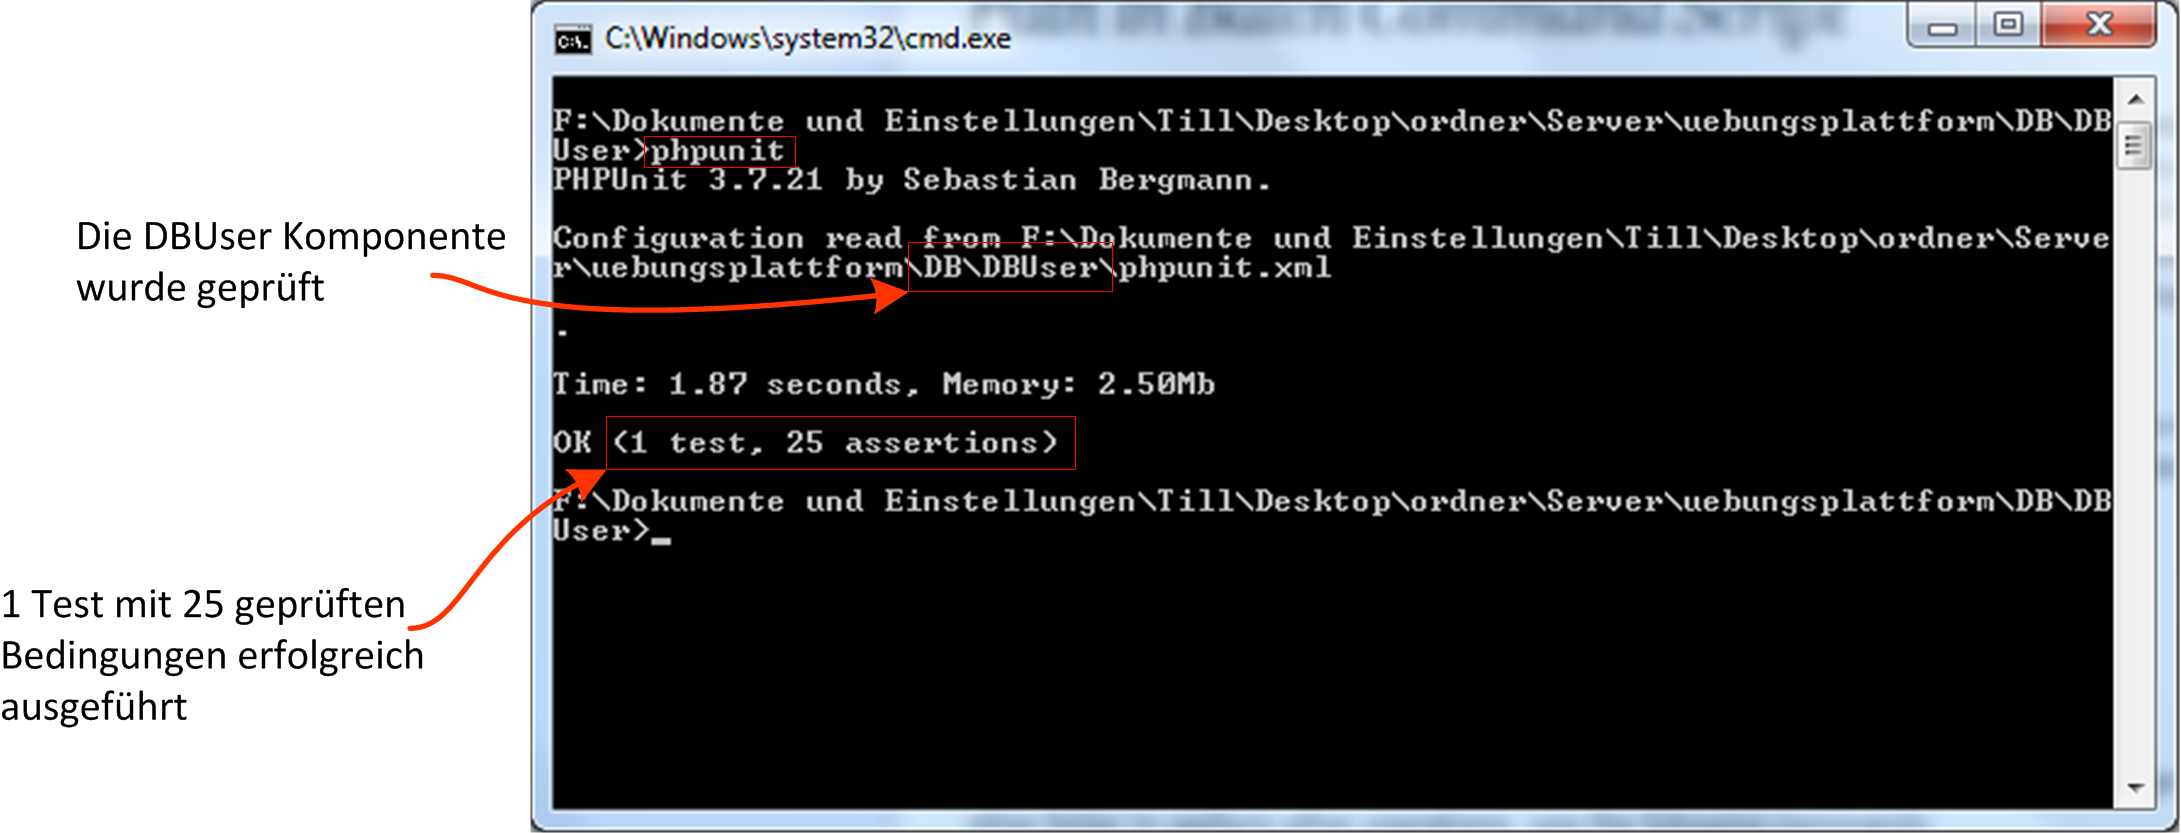
\includegraphics[scale=1]{Images/Testen.png}
  \end{minipage}\hfill

\subsubsection{Software}
  \begin{tabular}{l>{$}r<{$}}
\multirow{2}{.20\textwidth}{MySQL Server} & \multirow{2}{.70\textwidth}{Zum Betreiben der Datenbank (http://dev.mysql.com/downloads/mysql/)}\\& \\ \hline
\multirow{2}{.20\textwidth}{PHPUnit} & \multirow{2}{.70\textwidth}{Die Testumgebung (http://phpunit.de/)}\\&\\
 \end{tabular}

\subsubsection{Einstellungen}
Die Anfragegrundadresse für die HTTP Requests muss in der entsprechenden \blau{DB/phpunit.ini} eingestellt werden.

Beispielinhalt der \blau{phpunit.ini} Datei:

\begin{minipage}{\textwidth}
\begin{lstlisting}
[PHPUNIT]
// Die Anfrageadresse fuer die HTTP Requests
url = http://localhost/uebungsplattform/DB/ 
\end{lstlisting}
\end{minipage}
 
 \subsection{Der lange Weg zur neuen Komponente}
 \subsubsection{Entwickeln}
 Es muss sichergestellt werden, dass die Aufrufe dieser Komponente mittels REST möglich sind, dazu kann, sofern PHP zum Einsatz kommt, kann das Slim Framework genutzt werden, entsprechende Beispiele zur Nutzung können ebenfalls bereits bestehenden Komponenten entnommen werden. 
 
\begin{minipage}{\textwidth}
Beispiel:
\begin{lstlisting}
require_once( '../../Assistants/Slim/Slim.php' );
\Slim\Slim::registerAutoloader();
...
// initialisiert slim
$this->_app = new \Slim\Slim();

// Slim soll auf einen PUT Aufruf an diese Komponenten,
// mit der URI /course/:courseid die Funktion "editCourse"
// aufrufen und $courseid setzen.
// Bsp.: /course/1 oder /course/abc
$this->_app->put('/course/:courseid',
                 array($this,'editCourse'));
...

// hier wird die aufzurufende Funktion definiert
public function editCourse($courseid)
{
    ...
}
\end{lstlisting}
\end{minipage}

Daten, welche in die Komponenten hineingehen oder diese verlassen, sollten JSON kodiert sein. Dazu kann im Kapitel über Datenstrukturen nachgelesen werden.

Wir Antworten mit unserer Komponente nun indem wir mindestens den HTTP Statuscode und einen Body der Antwort setzen.

\begin{minipage}{\textwidth}
\begin{lstlisting}
public function editCourse($courseid)
{
    // setzt den Statuscode
    $this->_app->response->setStatus(201);

    // setzt den Inhalt der Antwort
    $this->_app->response->setBody('[]');
    
    // beendet diesen Aufruf sofort, gibt aber die 
    // festgelegte Antwort trotzdem zurueck
    $this->_app->stop();
}
\end{lstlisting}
\end{minipage}

Jede Komponente sollte so entworfen werden, das man sie komplett eigenständig betreiben kann, abgesehen von Hilfsdateien, welche sich mehrere Komponenten teilen.


 
 \subsubsection{Anbinden}
 Um die Komponente mit anderen zu verbinden müssen die entsprechenden Einträge in der Datenbank angelegt werden, dies kann entweder über die $CControl$ Komponente mittels entsprechender Kommunikation erfolgen oder über einen direkten Zugriff auf die Datenbanktabellen $Component$ und $ComponentLinkage$. 
 
Dabei muss ein neuer Eintrag für die Komponente in der $Component$ Tabelle erstellt werden, sodass sie eine ID erhält. Wollen wir nun die neue Komponente eine andere Aufrufen lassen können, so erstellen wir einen neuen $ComponentLinkage$ Eintrag und vermerken unsere neue ID dort als $CO\_id\_owner$, sowie die ID der Komponente die wir aufrufen können wollen als $CO\_id\_target$. Zudem wird der Linkname $CL\_name$ in der Komponente später genutzt um die Verwendung dieser Verknüpfung zu erklären oder verschiedene Ziele, sofern eine Komponente mehrere Ausgänge hat, zu unterscheiden.

So besitzen beispielsweise einige Komponenten Links mit dem Namen $Controller$ und wissen, damit, dass sie diese für Anfragen an einen Controller nutzen. Diese Namensvergabe ist jedoch Sache des Entwicklers der Komponente, es gibt dafür keine Festlegungen. Der häufigste Name ist dabei $out$, da meist kein besonderer Name benötigt wird.
 
Bei einer Änderung der Verknüpfungen sollten diese mit den unter Komponenten-Verknüpfung beschriebenen Schritten neu eingespielt werden.
  
\section{HTTP Requests erstellen}
Für HTTP-Requests nutzen wir cURL, dazu wurden Hilfsklassen entwickelt, welche den Zugriff darauf erlauben. Alles notwendige dazu finden wir in den Dateien \blau{Assistants/Request.php} und \blau{Assistants/Request/CreateRequest.php}.

\subsection{Anfragen für Anfänger}
\begin{minipage}{\textwidth}
\begin{lstlisting}
    public static function custom($method, 
                                  $target, 
                                  $header,  
                                  $content)
    {
        ...
    }
\end{lstlisting}
\end{minipage}

Dabei werden GET,PUT und POST unterstützt, zudem gibt es auch die Möglichkeit, eigene Methoden anzugeben.
\blau{Assistants/Request.php}

\begin{minipage}{\textwidth}
Beispiel:
\begin{lstlisting}
$ch = Request::custom(
                  'GET', // Methode
                  'http://.../DBCourse/course', // Anfrageziel
                  array(), // Header
                  ''); // Content
echo $ch['status'];
echo $ch['content']; 
                     
// Ausgabe: (nur beispielhaft)
//          200
//          []         
\end{lstlisting}
\end{minipage}
Auf den Header greifen Sie über \blau{\$ch['headers']} zu.

\subsection{Anfragen mit Verknüpfungen}
\begin{minipage}{\textwidth}
\begin{lstlisting}
    public static function routeRequest($method, 
                                        $resourceUri, 
                                        $header,  
                                        $content,
                                        $linkedComponents,
                                        $prefix,
                                        $linkName=NULL)
    {
        ...
    }
\end{lstlisting}
\end{minipage}

Wenn wir eine Liste von $Link$ Objekten zur Verfügung haben, so können wir die \blau{Request::routeRequest()} Funktion nutzen, um das Ziel unserer Anfrage aus mehreren Verknüpfungen suchen zu lassen.
\blau{Assistants/Request.php}

\begin{minipage}{\textwidth}
Beispiel:
\begin{lstlisting}
$ch = Request::routeRequest("GET", // Methode
                            '/course', // Anfrage-URI
                            array(), // Header
                            '', // Content
                            $links); // Linkliste
echo $ch['status'];
echo $ch['content']; 
                     
// Ausgabe: (nur beispielhaft)
//          200
//          []
\end{lstlisting}
\end{minipage}

\subsection{Anfragen mit SQL Dateien}
\begin{minipage}{\textwidth}
\begin{lstlisting}
    public static function getRoutedSqlFile($querys, 
                                            $sqlFile, 
                                            $vars,
                                            $checkSession=true)
    {
    	...
    }
\end{lstlisting}
\end{minipage}
Wenn wir eine Liste von $Link$ Objekten zur Verfügung haben und den Inhalt einer SQL Datei mit der Datenbank über die $DBQuery$ Komponente ausführen wollen, so können wir die \blau{DBRequest::getRroutedSqlFile()} Funktion nutzen.
Dabei können zusätzlich Variablen als Array übergeben werden, die dann innerhalb der SQL Datei global zur Verfügung stehen, da der Inhalt der SQL Datei mit PHP interpretiert wird über \blau{eval()}.

Es kann optional angegeben werden ob in der $Query$ Struktur, die zur $DBQuery$ Komponente geschickt wird, das Flag zur Prüfung der Session abgeschaltet werden soll.
\blau{Assistants/DBRequest.php}

\begin{minipage}{\textwidth}
Beispiel:
\begin{lstlisting}
$ch = DBRequest::getRoutedSqlFile($links, // Linkliste
                    'Beispiel.sql', // SQL Datei
                    array('userid' => $userid, // Platzhalter
                          'courseid' => $courseid),
                    false); // checksession ist hier aus
echo $ch['status'];
echo $ch['content']; 
                     
// Ausgabe: (nur beispielhaft)
//          200
//          []
\end{lstlisting}
\end{minipage}

\section{Den Logger nutzen}
Um Informationen nachvollziehbar speichern zu können, wurde eine Logger Klasse angelegt, diese ist zu finden unter \blau{Assistants/Logger.php}.

\begin{minipage}{\textwidth}
Beispiel:
\begin{lstlisting}
Logger::Log("ERROR Eintrag",LogLevel::ERROR);
Logger::Log("WARNING Eintrag",LogLevel::WARNING);
Logger::Log("INFO Eintrag",LogLevel::INFO);
Logger::Log("DEBUG Eintrag",LogLevel::DEBUG);
Logger::Log("Eigene Zieldatei",
            LogLevel::DEBUG, 
            "/var/www/ziel.log");
\end{lstlisting}
\end{minipage}
 
\section{Verteilerkomponenenten}
\subsection{Controller Klasse}
Um es anderen Arbeitsbereichen zu erleichtern, die Komponenten eines Bereiches anzusprechen, wurden zentrale Ansprechpunkte eingerichtet, diese werden als Controller bezeichnet.

Sie nehmen Anfragen entgegen und suchen den Empfänger, um anschließend den Erfolg oder Misserfolg an den Anfragenden zurück zuleiten.

Eine einfache Implementierung ist die \blau{Assistants/Controller.php}. Sowohl die Datenbankschicht (DB) mit der DBControl Komponente \blau{DB/DBControl} und das Dateisystem (FS) mit der FSControl Komponente \blau{FS/FSControl} nutzen diese Klasse. Dabei werden 401,404 und 406 Fehler von dahinter aufgerufenen Komponenten direkt weitergegeben und der Suchvorgang beendet, alle weiteren Fehlernummern werden zu einer 409 zusammengefasst.

Dabei werden Aufrufe wie:\\
\blau{http://localhost/uebungsplattform/DB/DBCourse/course}\\
\blau{http://localhost/uebungsplattform/DB/DBUser/user}\\
\blau{http://localhost/uebungsplattform/DB/DBMarking/marking}\\

vereinheitlicht zu:\\
\blau{http://localhost/uebungsplattform/DB/DBControl/course}\\
\blau{http://localhost/uebungsplattform/DB/DBControl/user}\\
\blau{http://localhost/uebungsplattform/DB/DBControl/marking}\\

\subsection{Logik Controller}
Eine weitere eigenständige Variante ist der LController des Logikbereichs unter \blau{logic/Controller}. Da dieser Aufrufe an zwei weitere Bereiche leiten muss, ist hier die Herangehensweise etwas anders.

\section{Probleme}
Es gibt Bereiche, auf die man eine Auge haben sollte, weil sie entweder nicht komplett sauber definiert wurden oder nicht klar ist, ob sie so funktionieren, wie sie sollen. Zudem sind dinge Aufgetreten, die einem das Entwickeln erschwert haben.

\subsection{Aufrufzeiten lokaler Komponenten}
Zum Aufruf andere Komponenten innerhalb des Systems wird cURL genutzt, dabei entstammen die meisten Aufrufe der 
\textcolor{blue}{Assistants/Request.php}. Bei jedem Aufruf einer lokalen Komponente verlieren wir einige Millisekunden zum Aufbau der Verbindung (etwa 20ms), eventuell muss daran gearbeitet werden, diesen Verlust durch entsprechende Serverkonfiguration zu kompensieren oder den Versuch unternehmen, den cURL Aufruf lediglich zu Simulieren und keine Verbindung über cURL Aufzubauen, wenn es sich um einen lokalen Aufruf handelt, sondern den PHP Code direkt auszuführen.

\subsection{Dateien löschen}
Für das löschen von Dateien muss sowohl die $File$ Tabelle der Datenbank als auch das Dateisystem betrachtet werden. Eine Datei kann erst aus dem Dateisystem gelöscht werden, wenn sie in der Datenbank nicht länger benötigt wird. Dazu prüft die Datenbank die Fremdschlüsselbedingungen, sodass sie das löschen eines Datenbankeintrages von selbst ablehnt, sofern dieser noch benötigt wird.

Da einige Tabellen Zeiger auf die $File$ Tabelle nutzen, beispielsweise enthält eine $Submission$ einen Zeiger auf eine Datei der $File$ Tabelle. Sodass theoretisch beim löschen einer Submission sowohl der $File$ als auch der $Submission$ Eintrag manuell gelöscht werden müssen.

Das Problem entsteht an der Stelle, wo $ExerciseSheet$ rekursiv im Fall des Löschens, seine $Submission$, $Marking$ und $Exercise$ automatisch aus der Datenbank entfernt, um selbst gelöscht zu werden (durch die Fremdschlüsselbedingungen).

Wird nun eine solche $Submission$ rekursiv beim löschen der $ExerciseSheet$ entfernt, geht der Verweis auf die $File$ Tabelle verloren und es kommt zu keinem sauberen Löschvorgang der Dateien aus der $File$ Tabelle und dem Dateisystem.

Eine Idee zur Lösung dieses Problems war es eine zusätzliche $RemovableFiles$ Tabelle anzulegen, in welche rekursiv entfernte $File$ Einträge verschoben werden. Sodass man diese Einträge abrufen und das Dateisystem bereinigen kann.

\subsection{Lange Aufrufzeiten, viele Anfragen}
- Aufbereitung der Daten \\
- neue gezieltere Anfragen in der DBL erstellen \\
- meist ist es schneller mehr abzufragen und Daten zu verwerfen, als mehrere kleine Anfragen zu stellen\\
\todo{aufschreiben}

\subsection{Requests funktionieren nicht im Uninetz}
- Firewalleinstellungen, \\
- GET mit Content/Postfield geht nicht\\
\todo{aufschreiben}

\end{document}